%% LaTeX-Beamer template for KIT design
%% by Erik Burger, Christian Hammer
%% title picture by Klaus Krogmann
%%
%% version 2.1
%%
%% mostly compatible to KIT corporate design v2.0
%% http://intranet.kit.edu/gestaltungsrichtlinien.php
%%
%% Problems, bugs and comments to
%% burger@kit.edu

\documentclass[18pt]{beamer}


%% SLIDE FORMAT

% use 'beamerthemekit' for standard 4:3 ratio
% for widescreen slides (16:9), use 'beamerthemekitwide'
\usepackage{listings}
\usepackage{templates/beamerthemekit}
% \usepackage{templates/beamerthemekitwide}
\usepackage{color}
\definecolor{editorGray}{rgb}{0.95, 0.95, 0.95}
\definecolor{editorOcher}{rgb}{1, 0.5, 0} % #FF7F00 -> rgb(239, 169, 0)
\definecolor{editorGreen}{rgb}{0, 0.5, 0} % #007C00 -> rgb(0, 124, 0)
\usepackage{upquote}
\lstdefinelanguage{JavaScript}{
	morekeywords={typeof, new, true, false, catch, function, return, null, catch, switch, var, if, in, while, do, else, case, break},
	morecomment=[s]{/*}{*/},
	morecomment=[l]//,
	morestring=[b]",
	morestring=[b]'
}

\lstdefinelanguage{HTML5}{
	language=html,
	sensitive=true, 
	alsoletter={<>=-},
	otherkeywords={
		% HTML tags
		<html>, <head>, <title>, </title>, <meta, />, </head>, <body>,
		<canvas, \/canvas>, <script>, </script>, </body>, </html>, <!, html>, <style>, </style>, ><
	},  
	ndkeywords={
		% General
		=,
		% HTML attributes
		charset=, id=, width=, height=,
		% CSS properties
		border:, transform:, -moz-transform:, transition-duration:, transition-property:, transition-timing-function:
	},  
	morecomment=[s]{<!--}{-->},
	tag=[s]
}

\lstset{%
	% Basic design
	backgroundcolor=\color{editorGray},
	basicstyle={\small\ttfamily},   
	frame=l,
	% Line numbers
	xleftmargin={0.75cm},
	numbers=left,
	stepnumber=1,
	firstnumber=1,
	numberfirstline=true,
	% Code design   
	keywordstyle=\color{blue}\bfseries,
	commentstyle=\color{darkgray}\ttfamily,
	ndkeywordstyle=\color{editorGreen}\bfseries,
	stringstyle=\color{editorOcher},
	% Code
	language=HTML5,
	alsolanguage=JavaScript,
	alsodigit={.:;},
	tabsize=2,
	showtabs=false,
	showspaces=false,
	showstringspaces=false,
	extendedchars=true,
	breaklines=true,        
	% Support for German umlauts
	literate=%
	{Ö}{{\"O}}1
	{Ä}{{\"A}}1
	{Ü}{{\"U}}1
	{ß}{{\ss}}1
	{ü}{{\"u}}1
	{ä}{{\"a}}1
	{ö}{{\"o}}1
}
%% TITLE PICTURE

% if a custom picture is to be used on the title page, copy it into the 'logos'
% directory, in the line below, replace 'mypicture' with the 
% filename (without extension) and uncomment the following line
% (picture proportions: 63 : 20 for standard, 169 : 40 for wide
% *.eps format if you use latex+dvips+ps2pdf, 
% *.jpg/*.png/*.pdf if you use pdflatex)

\titleimage{pink-blau}

%% TITLE LOGO

% for a custom logo on the front page, copy your file into the 'logos'
% directory, insert the filename in the line below and uncomment it

%\titlelogo{mylogo}

% (*.eps format if you use latex+dvips+ps2pdf,
% *.jpg/*.png/*.pdf if you use pdflatex)

%% TikZ INTEGRATION

% use these packages for PCM symbols and UML classes
% \usepackage{templates/tikzkit}
% \usepackage{templates/tikzuml}

% the presentation starts here

\title[CSS Basics]{CSS Basics}
\subtitle{Let's make things pretty!}
\author{Lena, Kristin, Charlotte}

% Bibliography

\usepackage[citestyle=authoryear,bibstyle=numeric,hyperref,backend=biber]{biblatex}
\addbibresource{templates/example.bib}
\bibhang1em

\begin{document}

% change the following line to "ngerman" for German style date and logos
\selectlanguage{ngerman}

%title page
\begin{frame}
\titlepage
\end{frame}

\section {Was ist CSS}
\begin{frame}{Was ist CSS}
\begin {itemize}
\item Styling für unsere Webseite
\item Stylen kann man zum Beispiel mit:
\begin{itemize}
\item Schriftgr"o"se
\item Hintergrundbild
\item Anordnung der Elemente
\end{itemize}
\end {itemize}
\end{frame}

\begin{frame}[fragile]{CSS für unsere Webseite}
\begin {itemize}
\item Datei \glqq style.css\grqq im gleichen Ordner wie unsere \glqq index.html\grqq anlegen
\item Einbinden der CSS-Datei in index.html Header mit:
\begin{lstlisting}
<head>
	...
	<link rel="stylesheet" type="text/css" href="style.css"/>
	...
</head>
\end{lstlisting}
\end {itemize}
\pause
\textbf{Jetzt kann's losgehen!}
\end{frame}

\begin{frame}[fragile]{CSS Syntax}
\begin {itemize}
\item Ein CSS-Eintrag ist immer so aufgebaut:
\begin{lstlisting}
Elementname {
  Styling-Name: Styling-Wert;
}
\end{lstlisting}
\item Stylen können wir
\begin{itemize}
\item Typen von HTML Elementen (div, h1, a, ...)
\item HTML Elemente mit bestimmten IDs
\item HTML Elemente einer bestimmten Klasse
\end{itemize}
\end {itemize}
\end{frame}

\begin{frame}[fragile]{Stylen eines HTML Typs - Hintergrundfarbe}
Wir wollen die Hintergrundfarbe unserer gesamten Seite ändern:
\begin {itemize}
\item HTML Typ: body
\item Styling-Name: background-color
\item Styling-Wert: rgb(66, 134, 244) \footnote{Google: Color Picker}
\pause
\item 
\begin{lstlisting}
body {
  background-color: red;
}
\end{lstlisting}
\end {itemize}
\end{frame}

\begin{frame}[fragile]{Stylen eines HTML Typs - Hintergrundbild}
Wir wollen ein Bild als Hintergrund unserer gesamten Seite ändern:
\begin {itemize}
\item HTML Typ: body
\item Styling-Name: background-image
\item Styling-Wert: url(''bilder/hintergrund/einBildName.png'');
\pause
\item 
\begin{lstlisting}
body {
  background-image: url("bilder/hintergrund/pink-blau.png");;
}
\end{lstlisting}
\end {itemize}
\end{frame}

\begin{frame}[fragile]{Aufgabe - Style Deinen Hintergrund!}
\begin {itemize}
\item Suche Dir ein cooles Hintergrundbild oder eine schöne Farbe aus
\item Stelle dieses Bild/Farbe als Hintergrund für Deine Webseite ein!
\end {itemize}
\end{frame}

\begin{frame}[fragile]{Stylen eines HTML Typs - Schriftart}
Jetzt wollen wir f"ur unseren Text eine coole Schriftart haben!
\begin {itemize}
\item HTML Typ: body
\item Styling-Name: font-family
\item Styling-Wert: 'Athiti', sans-serif; \footnote{Google: Font Family List}
\pause
\item 
\begin{lstlisting}
body {
  font-family: 'Athiti', sans-serif;
}
\end{lstlisting}
\end {itemize}
\end{frame}

\begin{frame}[fragile]{Stylen eines HTML Typs - Schriftgr"o"se}
Nun m"ochten wir die Schriftgr"o"se festlegen:
\begin {itemize}
\item HTML Typ: body
\item Styling-Name: font-size
\item Styling-Wert: 20px
\pause
\item 
\begin{lstlisting}
body {
  font-size: 20px;
}
\end{lstlisting}
\end {itemize}
\end{frame}

\begin{frame}[fragile]{Stylen eines HTML Typs - Textanordnung}
Abschlie"send m"ochten wir die Ausrichtung der Schrift ver"andern
\begin {itemize}
\item HTML Typ: body
\item Styling-Name: text-align
\item Styling-Wert: center oder block oder left oder right
\pause
\item 
\begin{lstlisting}
body {
  text-align: center;
}
\end{lstlisting}
\end {itemize}
\end{frame}

\begin{frame}[fragile]{Aufgabe - Style Deine Schrift!}
\begin {itemize}
\item Suche Dir eine coole Schriftart, -gr"o"se und -ausrichtung aus und setze sie als ''body'' CSS Wert
\item Suche Dir eine andere Schriftart und -gr"o"se aus und setze sie f"ur alle h1 Elemente
\item Schaue Dir deine Webseite an. Was ist passiert? 
\end {itemize}
\end{frame}

\begin{frame}[fragile]{Stylen einer Klasse - Inhalt}
\begin{itemize}
\item Wir wollen unserer Webseite Struktur geben
\item Daf"ur packen wir den eigentlichen Inhalt der Webseite in ein div
\item Um das div separat zu stylen, geben wir ihm die Klasse inhalt
\begin{lstlisting}
<body>
	<div class="inhalt">
	...
	</div>
</body>
\end{lstlisting}
\pause
\item In der style.css Datei k"onnen wir inhalt jetzt stylen mit
\begin{lstlisting}
.inhalt {
  Styling-Name: Styling-Wert;
}
\end{lstlisting}
\end{itemize}
\end{frame}

\begin{frame}[fragile]{Aufgabe - Style den Inhalt!}
\begin{itemize}
\item Packe den Inhalt Deiner Webseite in ein div und gebe ihm eine Klasse ''inhalt''
\item Gib ''inhalt'' in der style.css einen anderen Hintergrund als ''body''
\item Lade deine Webseite neu. Was siehst Du?
\end{itemize}
\end{frame}

\begin{frame}[fragile]{Elementgr"o"sen - Width und Height}
\begin{itemize}
\item Um die Gr"o"se eines Elementes zu beeinflussen k"onnen wir Werte f"ur ''width'' (Breite) und ''height'' (H"ohe) setzen.
\item Das geht sowohl absolut mit Anzahl Pixeln, als auch relativ als Prozentzahl
\begin{lstlisting}
.inhalt {
  width: 600px;
  height: 100%
}
\end{lstlisting}
\end{itemize}
\end{frame}

\begin{frame}[fragile]{Abst"ande - Margin, Padding und Co}
\begin{itemize}
\item Um den Abstand des Elements zu anderen zu manipulieren, gibt es die CSS Eigenschaften
\begin{itemize}
\item margin: Au"senabstand
\item border: Rahmengr"o"se
\item padding: Innenabstand
\end{itemize}
\item F"ur jede Eigenschaft gibt es vier Werte: \\
top (oben), right (rechts), bottom (unten), left (links)
\end{itemize}
\end{frame}

\begin{frame}[fragile]{Abst"ande - Margin, Padding und Co}
\begin{figure}
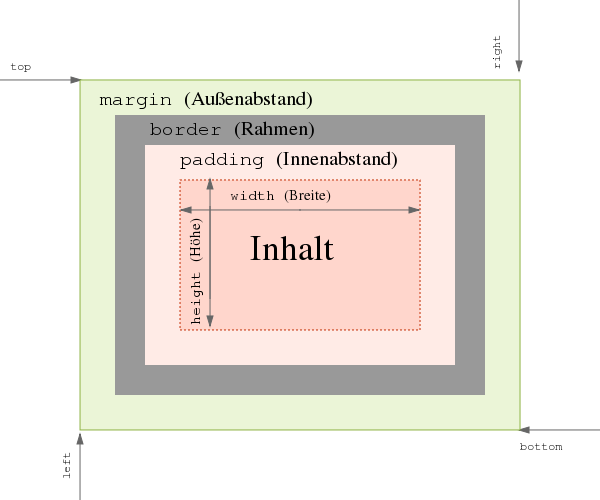
\includegraphics[width=0.8\textwidth]{600px-Box-Modell} %TODO: evtl selbst machen, Urheberrecht? Plus left.. sind komisch erklaert
\end{figure}
\end{frame}

\begin{frame}[fragile]{Abst"ande - Margin, Padding und Co}
Klingt kompliziert?
\pause
\begin{itemize}
\item "Offne Deine Webseite im Browser
\item Klicke F12
\item Probiere es aus!
\end{itemize}
\end{frame}

\begin{frame}[fragile]{Aufgabe - Style Deine Webseite!}
\begin{itemize}
\item Probiere verschiedene Werte f"ur die Abst"ande und Gr"o"sen von ''body'' und ''inhalt'' aus
\item Baue Deine Favoriten in deine Webseite ein!
\end{itemize}
\end{frame}


\begin{frame}[fragile]{Es ist wundersch"on!}
\begin{figure}

\includegraphics[height=0.8\textheight]{beautiful} 
\end{figure}
\end{frame}

\end{document}
